\documentclass[beamer]{standalone}
\usepackage{circuitikz}
\begin{document}

\title[Electronics 1]{Useful Circuits with Opamps}

\begin{frame} 
  \titlepage
\end{frame}

\section{Integrators}
\begin{frame}
\frametitle{Integrator}
\begin{figure}
	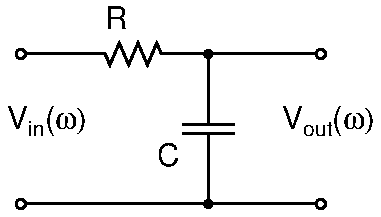
\includegraphics[width=0.40\textwidth]{./schematics/rc_low_pass.pdf}
\end{figure}
\[
V_{out}(t)=V_c(t)= \frac{Q(t)}{C} = \int \frac{I(t)}{C} dt 
= \int \frac{V_{in}(t)-V_c(t)}{RC} dt 
\]
\begin{block}{for $V_c \approx 0$}
\[
V_{out}(t) \approx \frac{1}{RC}\int V_{in}(t) dt
\]
\end{block}
\end{frame}

\begin{frame}[t]
\frametitle{Integral representation in Fourier space}
\begin{eqnarray*}
F(t) 
&=& \int^t_{-\infty} f(t') dt' 
=  \int^t_{-\infty} dt' \int^{+\infty}_{-\infty} f(\omega) e^{  i \omega t'} d\omega \\
&=&  \int^{+\infty}_{-\infty} d\omega \int^{t}_{-\infty} f(\omega) e^{  i
\omega t'} dt' \\
&=&  \int^{+\infty}_{-\infty} d\omega \left[ \frac{ f(\omega) }{ i \omega} e^{
i \omega t'}  {\Big|}^t_{-\infty} \right] \\
&=&  \int^{+\infty}_{-\infty} d\omega  \frac{ f(\omega) }{ i \omega} e^{
i \omega t} 
=  \int^{+\infty}_{-\infty} d\omega   F(\omega)  e^{ i \omega t} 
\end{eqnarray*}
\begin{columns}<2>
\begin{column}{0.5\textwidth}
\begin{eqnarray*}
F(t) &=& \int^t_{-\infty} f(t') dt' \\
F(\omega) &=&  \frac{ f(\omega) }{ i \omega}
\end{eqnarray*}
\end{column}
\begin{column}{0.5\textwidth}
\begin{eqnarray*}
G(t) &=& \frac{d g}{d t} \\
G(\omega) &=&   i \omega g(\omega)
\end{eqnarray*}
\end{column}
\end{columns}
\end{frame}

\begin{frame}
\frametitle{Integrator}
\begin{figure}
	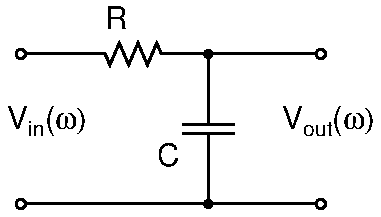
\includegraphics[width=0.40\textwidth]{./schematics/rc_low_pass.pdf}
\end{figure}
\[
V_{out}(\omega)=G(\omega) V_{in}(\omega)=\frac{Z_c}{R+Z_c}V_{in}(\omega)=\frac{1}{1+i\omega R C}V_{in}(\omega)
\]
\begin{block}{for $\omega \gg \omega_{3dB}$}
\[
V_{out}(\omega) \approx \frac{1}{R C} \frac{V_{in}(\omega)}{i \omega}
\]
\end{block}
\end{frame}

\frame
{ \frametitle{True Integrator / low-pass filter}
We need to keep 
\[
I=\frac{V_{in}}{R}
\]
\begin{figure}
	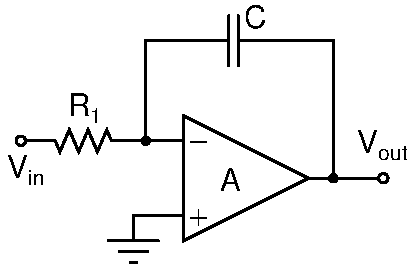
\includegraphics[width=0.40\textwidth]{./schematics/integrator.pdf}
\end{figure}
\[
G(\omega)=-\frac{Z_c}{R_1}=-\frac{1}{i\omega R_1 C}
\]
Only one problem remains: if any DC voltage is applied at input, output
will reach a rail at power supply voltage.

This can be thought as a lack of feedback since at DC capacitor blocks
everything.
	}

\frame
{ \frametitle{Low-pass filter / Integrator improved }
\begin{figure}
	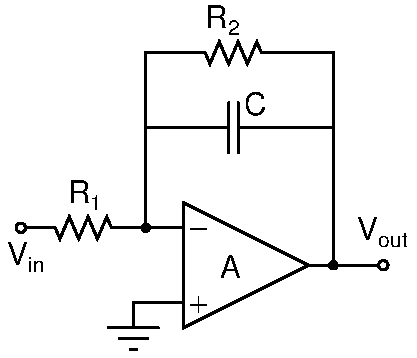
\includegraphics[width=0.40\textwidth]{./schematics/integrator_compensated.pdf}
\end{figure}
\[
G(\omega)=-\frac{Z_c\|R_2}{R_1}=-\frac{R_2}{R_1} \frac{1}{1+i\omega R_2 C}
\]
	}


\section{Differentiator}
\frame
{ \frametitle{Differentiator / high-pass filter}
\begin{figure}
	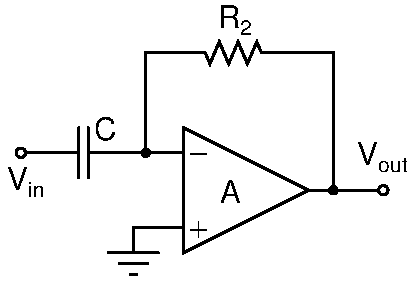
\includegraphics[width=0.20\textwidth]{./schematics/differentiator.pdf}
\end{figure}
\begin{eqnarray*}
	V_{in} &=&  \frac{Q}{C}=\frac{1}{C} \int I dt \to I= C \frac{dV_{in}}{dt}
	\\
	V_{out} &=&  - I R_2
\end{eqnarray*}
\begin{block}{}
\[
V_{out} = -R_2 C \frac{dV_{in}}{dt}
\]
\end{block}

\begin{block}{Fourier space}
\[
V_{out}(\omega) = -\frac{Z_{R_2}}{Z_c}= - i \omega R_2 C V_{in}(\omega)=
\omega R_2 C  V_{in}(\omega) e^{-i\frac{\pi}{2}}
\]
\end{block}

	}

\frame
{ \frametitle{Differentiator compensated}
\begin{figure}
	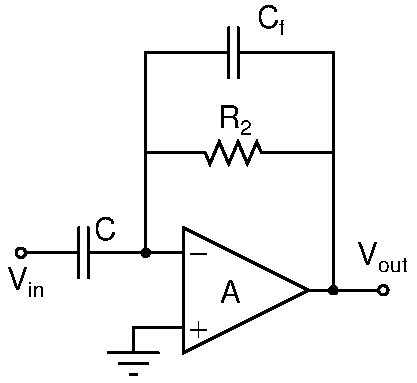
\includegraphics[width=0.25\textwidth]{./schematics/differentiator_compensated.pdf}
\end{figure}

\begin{block}{}
	\[
	V_{out}(\omega) = -\frac{Z_{R_2}\|Z_f}{Z_c}  V_{in}(\omega) =  - \frac{i \omega R_2 C} {1+ i\omega R_2 C_f} V_{in}(\omega)
	\]
\end{block}
\begin{columns}[t]
	\begin{column}{.45\textwidth}
		\begin{block}{$\omega \ll \frac{1}{R_2 C_f}$}
			\[
			V_{out}(\omega) = - {i \omega R_2 C} V_{in}(\omega)
			\]
		\end{block}

	\end{column}
	\begin{column}{.45\textwidth}
		\begin{block}{$\omega \gg \frac{1}{R_2 C_f}$}
			\[
			V_{out}(\omega) = - \frac{C}{C_f} V_{in}(\omega)
			\]
		\end{block}

	\end{column}
\end{columns}


}

\section{Functional feedback}
\frame{
\frametitle{Functional feedback}
\begin{figure}
	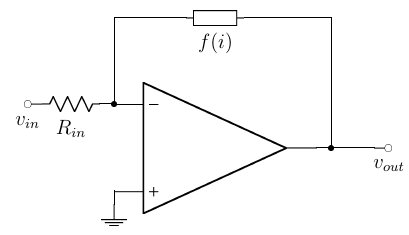
\includegraphics[width=0.5\textwidth]{./pics/functional}
\end{figure}

\begin{block}{}
\begin{eqnarray*}
 i(v_{diode}) & = & I_S (e^{v/V_T} - 1) \\
 v_{diode}(i) & = & \ln(1 + i/I_S)
\end{eqnarray*}
\end{block}

}

\section{Compensated thermistor}
\frame
{ \frametitle{Thermistor linearization}
\[
R_{th}(T)=R_0 e^{-\gamma (T-T_0)}
\]
Where $\gamma=0.04$, $T_0=20$~$^\circ$C, $R_0=10$~kOhm.
Below circuit linearizes the output 
voltage vs temperature ($R=R_0$ as an example).
\begin{columns}[c]
	\begin{column}{.25\textwidth}
		\begin{figure}
			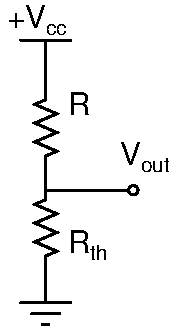
\includegraphics[width=0.80\textwidth]{./schematics/thermistor_linearization.pdf}
		\end{figure}
		
	\end{column}
	\begin{column}{.75\textwidth}
		\begin{figure}
			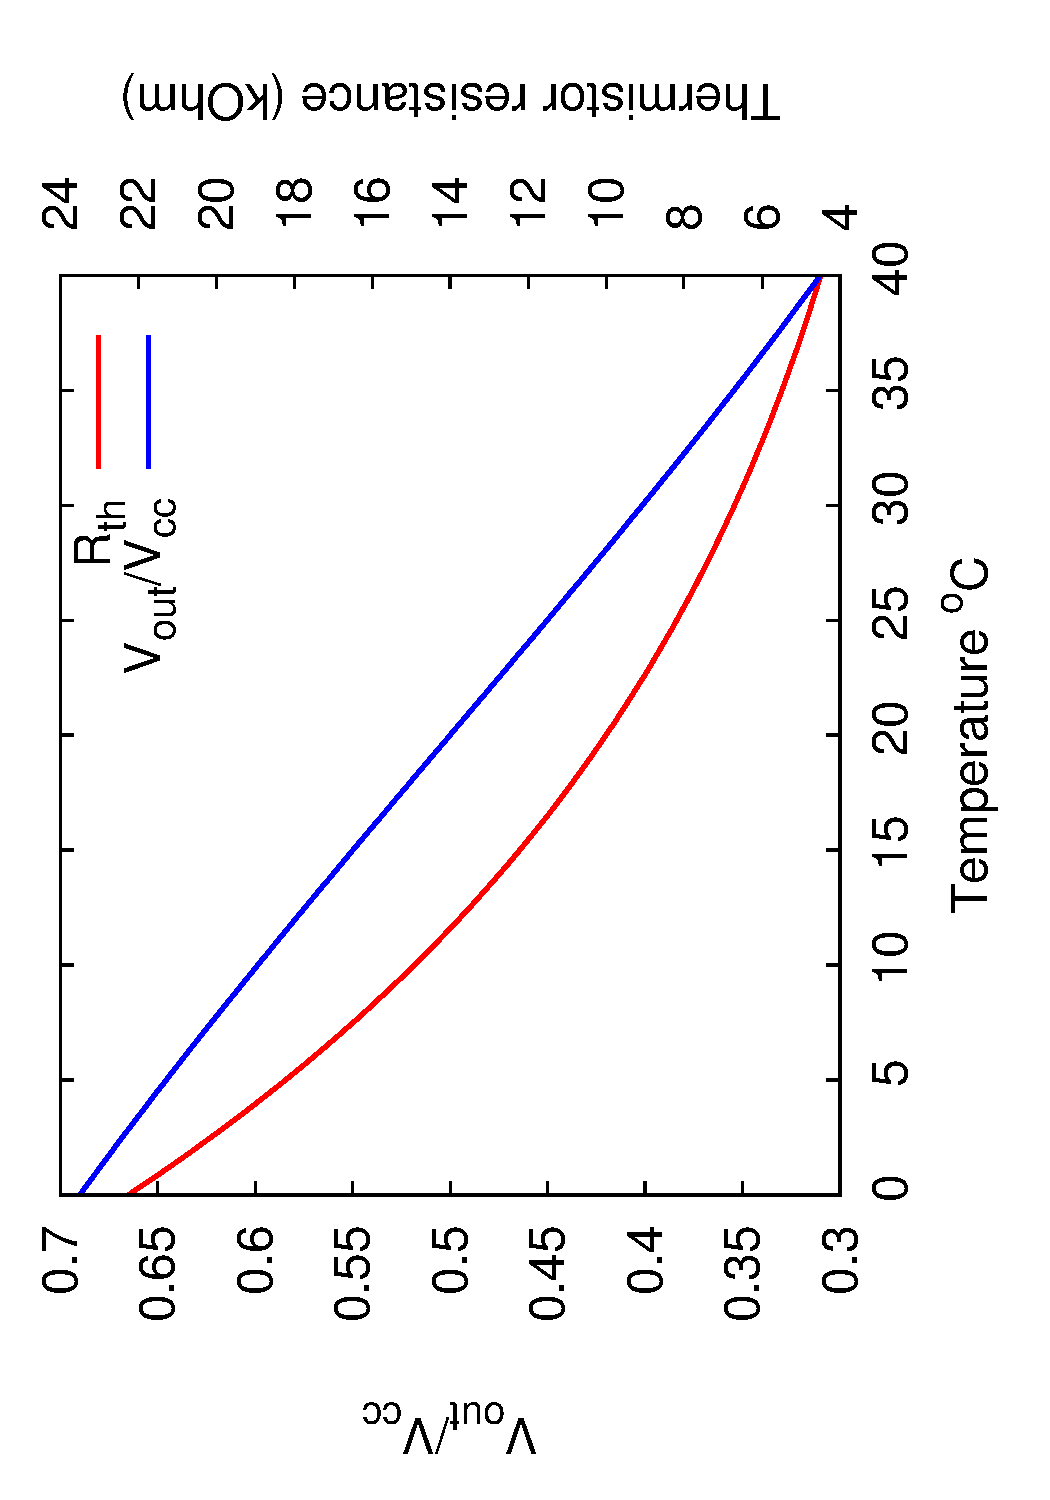
\includegraphics[angle=-90,width=0.80\textwidth]{./plots/thermistor_linearized.pdf}
		\end{figure}
	\end{column}
\end{columns}
	}
	
\end{document}
